\documentclass[chinese]{chemistry}

\begin{document}

\title{普通化学初步讲义\\[0.5em]
       \large\textit{第 1--3 章，待续}}

\author{Jiaming Shi\\[0.3em]
        \small Department of Physics, Westlake University\\
        \small\texttt{jiamingshi\_git@outlook.com}}

\date{\today}
\maketitle

\tableofcontents

\section{化学热力学}
\subsection{热力学的基本概念}
\begin{definition}[热力学系统]
热力学系统是指选定用于实验或理论研究的特定部分。系统之外一切其余部分定义为环境，而宇宙则是系统与环境的总和。
\end{definition}

根据系统与环境之间的物质和能量交换，可将系统分为以下几类：
\begin{enumerate}
    \item 敞开系统：与环境同时交换物质和能量；
    \item 封闭系统：与环境交换能量但不交换物质；
    \item 孤立系统：与环境既不交换物质也不交换能量。
\end{enumerate}

若描述系统的所有宏观物理性质都具有唯一确定的值，则称该系统处于确定的状态状态函数是指变化仅取决于系统的始态和终态，而与变化途径无关的物理量（例如 $V$、$T$、$p$）。

广延量是对各子系统具有加和性的状态函数（例如体积 $V$、物质的量 $n$、内能 $U$）。强度量是不具有加和性且与系统大小无关的状态函数，通常为两个广延量的比值（例如压力 $p$、温度 $T$、密度 $\rho$）。

过程量为非状态函数，其变化取决于系统状态变化的途径。

确定研究的系统后，我们可以像分析力学那样从能量的角度考虑其与环境的相互作用。我们将系统或环境的总能量称为热力学能（$U$），也称为内能，其绝对量不可知。

当两个系统处于热接触状态时，若它们之间没有净的能量传递，则称这两个系统处于热平衡状态。

\begin{proposition}[热力学第零定律]
若两个系统分别与第三个系统处于热平衡，则这两个系统彼此也处于热平衡。换句话说，这定义划分了一个等价类。
\end{proposition}
由于热平衡是等价关系，我们可以为每个等价类分配唯一的数值，这个数值就是我们所说的 温度（$T$）。

基于温度，系统与环境之间的相互作用可分为两类：一类由温度差引起，我们称之为热（$Q$），其余部分则为功（$W$）。显然，它们都不是状态函数。


绝热过程被定义为允许功但是不允许热的过程。

\begin{proposition}[热力学第一定律]
封闭系统的内能变化等于外界对系统所做的功与系统吸收的热之和，核心公式为：$$\Delta U = U_f - U_i = W + Q$$ 
其微分形式为：（注：d 仅用于状态函数，$\delta$仅为无穷小量的标记）
$$dU = \delta W +\delta Q $$
其中 $\Delta U$ 为内能变化，$U_f$ 和 $U_i$ 分别为系统的终态和始态内能。$W$ 为功，$Q$ 为热，符号上，系统获得能量时，$W$ 和 $Q$ 取正值；系统失去能量时，取负值。
\end{proposition}

对于宇宙而言，不存在环境，此时：
$$W=Q=0$$ 
即 $U$ 为常数，换句话说，宇宙的能量是守恒的。

接下来我们可以分别研究功和热。

最重要的一类功是体积功（$W_e$），也称为膨胀功，其定义为系统因体积变化对抗外压所做的功（或外界对系统做的功），遵循力学中功的基本定义 $\delta W=F dr$。注意到力和压强、体积和位矢之间的关系：
$$F = - p S, \quad dV = S dr$$ 
可得：

\begin{proposition}[体积功]
$$\delta W_e = -p_{ex}dV, \quad W_e = \int_{V_1}^{V_2} -p_{ex}dV$$
其中 $p_{ex}$ 为外压，$dV$ 为系统的体积无穷小变化。对于理想气体，典型可逆过程的体积功为：
\begin{enumerate}
    \item 恒压过程（$p_{ex}=\text{常数}$）：$W_e = -p(V_2 - V_1)$；
    \item 恒温过程（$T=\text{常数}$）：$W_e = - \nu RT\ln\frac{V_2}{V_1}$；
    \item 恒容过程（$V=\text{常数}$）：$W_e = 0$。
\end{enumerate}
\end{proposition}

我们将其余的所有功称为非体积功（$W_f$），将在后续章节中研究。本章中假设不存在非体积功。

首先是关于恒容状态的，在这种情况下$W = W_e + W_f = 0$，结合热一律，$\Delta U = Q + W = Q$，我们用记号$Q_V$来指示恒容状态:

\begin{definition}[恒容（反应）热]
对于仅存在体积功（$W_f=0$）的封闭系统，其在恒容条件下吸收或放出的热（$Q_V$）称为恒容热，其大小等于系统的内能变：$Q_V = \Delta U$。
\end{definition}

对于恒压过程，我们对体积功的计算，给出了$\Delta U = U_f - U_i = W + Q =Q - p_{ex} (V_f - V_i )$，整理得：$$Q =(U_f + p_{ex} V_f ) - (U_i + p_{ex} V_i)$$我们发现量$U + p V$指示了热，于是定义：

\begin{definition}[焓（恒压（反应）热）]
焓（$H$）是定义为 $H = U + pV$ 的状态函数，其状态函数的性质由Hess（盖斯）定律指出。显然，其绝对量也不可知。

对于仅存在体积功（$W_f=0$）的封闭系统，其在恒压条件下吸收或放出的热（$Q_p$）称为恒压热，其大小等于系统的焓变：$Q_p = \Delta H$。
\end{definition}

\begin{proposition}[焓变与内能变化的关系]
对于涉及气体的反应，焓变与内能变化的关系为：
$$\Delta H = \Delta U + \Delta \nu_g RT$$
其中 $\Delta \nu_g = \sum \nu(\text{气体产物}) - \sum \nu(\text{气体反应物})$ 为反应前后气态物质的物质的量变化。
\end{proposition}

绝大多数的化学反应体系都是恒压的，所以我们着重讨论焓。由于焓的绝对量不可知，我们定义一个标准：

\begin{definition}[标准摩尔生成焓、燃烧焓与键焓]
\begin{enumerate}
    \item 标准摩尔生成焓（$\Delta_f H_m^\circ$）：在指定温度（通常为298.15 K）下，由最稳定的单质在标准状态下生成1摩尔纯物质时的焓变。
    \item 标准摩尔燃烧焓（$\Delta_c H_m^\circ$）：在指定温度下，1摩尔纯物质完全燃烧生成标准状态下的稳定氧化物时的焓变。
    \item 键焓（键解离能）（$BDE$）：在指定温度下，1摩尔某化学键断键的焓变。
\end{enumerate}
\end{definition}

从定义可以看出，焓是温度的函数，由于热容变化贡献（$\int C_p \,dT$）。当然，这不在普化的讨论范围。

在这些式子中，我们引入大量的角标，$\Delta$的角标代表对变化过程的描述，例如$f$为生成、$r$为反应等等；函数的角标$m$代表“每摩尔”，更准确来说是偏摩尔量，$H_{m,i} = \left( \frac{\partial H}{\partial n_i} \right)_{T, p, n_j (j \neq i)}$；而上标$^\circ$为标准状态，$p_i = 1 \text{bar}$，$c_i = 1 \text{M} $。

结合Hess定律，我们很容易给出：

\begin{proposition}[化学反应的焓变]
化学反应的标准偏摩尔焓变可通过以下公式计算：
$$\Delta_r H_m^\circ = \sum \nu \Delta_f H_m^\circ(\text{产物}) - \sum \nu \Delta_f H_m^\circ(\text{反应物})$$
$$\Delta_r H_m^\circ = \sum \nu \Delta_c H_m^\circ(\text{反应物}) - \sum \nu \Delta_c H_m^\circ(\text{产物})$$
也可通过键解离能估算：$\Delta_r H_m = \sum BDE(\text{反应物}) - \sum BDE(\text{产物})$
\end{proposition}

\subsection{化学反应的自发性}

热机是将热能转化为功的装置，Carnot（卡诺）热机是典型的热机，其由两个等温过程和两个绝热可逆过程组成的可逆循环，工作在高温热源$T_h$和低温热源$T_c$之间。热力学给出了：

\begin{proposition}[Carnot定理]
$$\eta = \frac{W}{Q_{in}} \leq 1 - \frac{T_c}{T_h}$$
其中$Q_{in}$ 为从高温热源吸收的热，$W$ 为热机对外做的功。
\end{proposition}

结合能量守恒 $Q_{in} = W + Q_{ex}$（$Q_{ex}$ 为向低温热源放出的热），可得：
$$\frac{-Q_{ex}}{T_c} + \frac{Q_{in}}{T_h} \geq 0$$


\begin{definition}[熵]
熵（$S$）是描述系统混乱度的状态函数，其可逆过程的微分定义为：
$$dS = \frac{\delta Q_{rev}}{T}$$
\end{definition}

带入即给出了$dS_{total} = dS_{sur} + dS_{sys} \geq 0$， 即：

\begin{proposition}[熵增原理（热力学第二定律等价表述）]
对于孤立系统，自发过程中熵永不减少：
$$\Delta S \geq 0$$
其中可逆过程 $\Delta S = 0$，不可逆过程 $\Delta S > 0$。
\end{proposition}

对于非孤立恒压系统，我们开始推导其自发性条件，$dS_{total} = dS_{sur} + dS_{sys}$，我们认为环境为可逆，带入熵的定义与热一律，整理得：

$$T dS_{total} = \delta W - dU + T dS_{sys} \geq 0 $$

结合体积功与焓的定义，给出：

$$dH - T dS_{sys} \leqslant 0 $$

\begin{definition}[Gibbs自由能（Gibbs-Helmholtz方程）]
Gibbs（吉布斯）自由能（$G$）是定义为 $G = H - TS$ 的状态函数，其中 $H$ 为焓，$T$ 为热力学温度，$S$ 为熵。对于恒温恒压无非体积功的过程，热力学自发性判据为：
$$dG < 0 \ (\text{自发过程}),\quad \ dG = 0 \ (\text{平衡状态}),\quad \ dG > 0 \ (\text{非自发过程})$$
当然，这是热力学上的，并不代表一定（收到动力学限制）。
\end{definition}

当然，涉及非体积功时：

\begin{proposition}[热力学允许条件]
$$\Delta_r G_m < W_f$$
从这里可以看出，Gibbs自由能衡量了体系对外做非体积功的能力。
\end{proposition}



从气体出发并推广，van't Hoff(范特霍夫)给出了偏摩尔Gibbs自由能随浓度（反应商）变化的方程：

\begin{definition}[浓度商]
对于一般反应 $aA + bB \rightleftharpoons cC + dD$，反应商为：
$$Q_c = \frac{\left(\frac{[C]}{c^\circ}\right)^c \left(\frac{[D]}{c^\circ}\right)^d}{\left(\frac{[A]}{c^\circ}\right)^a \left(\frac{[B]}{c^\circ}\right)^b},\quad Q_p = \frac{\left(\frac{[C]}{p^\circ}\right)^c \left(\frac{[D]}{p^\circ}\right)^d}{\left(\frac{[A]}{p^\circ}\right)^a \left(\frac{[B]}{p^\circ}\right)^b}$$
其中 $c^\circ = 1M$ 为标准浓度，$p^\circ = 1bar$ 为标准分压，$[\cdot]$ 为物质的摩尔浓度或分压。
\end{definition}

\begin{proposition}[van't Hoff等温等压方程]
反应的偏摩尔Gibbs自由能变（$\Delta_r G_m$）与其标准偏摩尔Gibbs自由能变（$\Delta_r G_m^\circ$）和反应商（$Q$）的关系为：
$$\Delta_r G_m = \Delta_r G_m^\circ + RT\ln Q$$
\end{proposition}

显然，标准偏摩尔Gibbs自由能是在各组分浓度或分压在标准值时的偏摩尔Gibbs自由能变，可以判断各组分浓度或分压在标准值时反应的自发性。对任意时刻，我们应该考虑的是此时的$dG$或者此时反应商对应的偏摩尔Gibbs自由能变。

\subsection{化学平衡}

化学平衡是自发性问题的特殊情况。



从之前的推导可以得出，体系达到平衡状态时，其摩尔Gibbs自由能变等于0，我们将此时的反应商定义为标准平衡常数$K^\circ$。

\begin{proposition}[标准平衡常数]
化学平衡时，反应的摩尔Gibbs自由能变为零（$\Delta_r G_m=0$），因此标准平衡常数（$K^\circ$）满足：
$$\Delta_r G_m^\circ = -RT\ln K^\circ$$
结合Gibbs-Helmholtz方程，可得van't Hoff方程：
$$\ln K^\circ = -\frac{\Delta_r H_m}{R} \cdot \frac{1}{T} + \frac{\Delta_r S_m}{R}$$
\end{proposition}

我们将标准平衡常数带入van't Hoff等温等压方程，给出：

\begin{proposition}[反应方向判断]
恒温恒压下化学反应的方向由 $\Delta_r G_m$ 的符号决定，其与反应商（$Q$）和平衡常数（$K^\circ$）的比值关系为：
$$\Delta_r G_m = RT\ln\frac{Q}{K^\circ}$$
\begin{enumerate}
    \item $Q < K^\circ$：$\Delta_r G_m < 0$，正反应自发；
    \item $Q = K^\circ$：$\Delta_r G_m = 0$，系统处于化学平衡；
    \item $Q > K^\circ$：$\Delta_r G_m > 0$，逆反应自发。
    \end{enumerate}
\end{proposition}

现在，我们终于可以从能量的范围，用温度与浓度（分压）讨论化学平衡。

我们先讨论较为简单的恒容体系。

条件对化学平衡的影响可以分为两类，一类是直接改变了平衡常数，一类是改变了物质的浓度。

\begin{proposition}[温度对平衡的影响]
温度对化学平衡的影响由反应焓变（$\Delta_r H_m$）的符号决定：
\begin{enumerate}
    \item 吸热反应（$\Delta_r H_m > 0$）：升高温度使 $K^\circ$ 增大，平衡正向移动；
    \item 放热反应（$\Delta_r H_m < 0$）：升高温度使 $K^\circ$ 减小，平衡逆向移动。
\end{enumerate}
$\ln K^\circ$ 对 $1/T$ 作图为一条直线，斜率为 $-\Delta_r H_m/R$，截距为 $\Delta_r S_m/R$。
\end{proposition}

不难发现，升高温度会使反应向吸热的方向发展，以试图降低温度。

\begin{proposition}[浓度和惰性气体对平衡的影响]
\begin{enumerate}
    \item 加入反应物使其浓度增大，$Q < K^\circ$，平衡正向移动；加入产物使其浓度增大，$Q > K^\circ$，平衡逆向移动。
    \item 加入惰性气体无影响（浓度不变）。
\end{enumerate}
\end{proposition}

同样的，体系试图消耗新引入的物质。

对于非恒容过程，其平衡的讨论时极其复杂的，因为条件的改变可能同时改变了体积，导致浓度的变化，在极端情况下造成刚好相反的效果。其中最简单的就是直接改变压强（体积）。

\begin{proposition}[体积和压力对平衡的影响]
对于气相反应 $a\text{A}(g) + b\text{B}(g) \rightleftharpoons c\text{C}(g) + d\text{D}(s)$，气态物质的物质的量变化为 $\Delta n(g) = c - a - b$。反应商可表示为：
$$Q = \frac{n^c([\text{C}])}{n^a([\text{A}])n^b([\text{B}])} \cdot V^{-\Delta n(g)}$$
其中 $V$ 为系统体积。改变体积（或压力）会改变 $Q$ 的值：
\begin{enumerate}
    \item 减小体积（增大压力）：若 $\Delta n(g) > 0$，$Q$ 增大，平衡逆向移动；若 $\Delta n(g) < 0$，$Q$ 减小，平衡正向移动；
    \item 增大体积（减小压力）：变化趋势与减小体积相反；
    \item $\Delta n(g) = 0$：体积/压力变化对平衡无影响。
\end{enumerate}
\end{proposition}

上述表达式的证明如下：

$$a\text{A}(g) + b\text{B}(g) \rightleftharpoons c\text{C}(g) + d\text{D}(s)$$
其浓度商为：
$$Q = \frac{\left(\frac{[\text{C}]}{c^\circ}\right)^c \left(\frac{[\text{D}]}{c^\circ}\right)^d}{\left(\frac{[\text{A}]}{c^\circ}\right)^a \left(\frac{[\text{B}]}{c^\circ}\right)^b} = \frac{\left(\frac{n_{\text{C}}}{V c^\ominus}\right)^c}{\left(\frac{n_{\text{A}}}{V c^\ominus}\right)^a \left(\frac{n_{\text{B}}}{V c^\ominus}\right)^b}$$
整理得：
$$Q = \frac{n_{\text{C}}^c}{n_{\text{A}}^a n_{\text{B}}^b} \cdot V^{-\Delta n(g)}$$

\begin{proposition}[浓度和惰性气体对平衡的影响]
\begin{enumerate}
    \item 加入惰性气体相当于增大体积，平衡移动遵循体积变化的规律；
    \item 加入反应物/产物会同时引起体积变化，移动方向由各个物质浓度共同决定。
\end{enumerate}
\end{proposition}

\begin{example}[加入反应物平衡逆移的例子]
我们考察这样的一个反应：
$$\text{Cl}_2(g) + \text{PCl}_3(g) \rightleftharpoons  \text{PCl}_5(g)，\quad K = 26$$
假设原先处于体积为1$\mathrm{L}$的体系，$\text{Cl}_2$和$\text{PCl}_3$的浓度都是1$\mathrm{M}$，显然，$\text{PCl}_5$的浓度为26$\mathrm{M}$。

现在，我们向这个体系加入99$\mathrm{mol}$的$\text{Cl}_2$。设反应正向进行了$x \mathrm{mol}$，计算各个物质浓度，代入$K_c$，约去体积得：

$$\frac{(26+x)(127-x)}{(1-x)(100-x)} = 26 \implies x \approx -0.26\ \mathrm{mol}$$

$$n(\text{PCl}_5) = 26 - 0.26 = 25.74\ \mathrm{mol}$$
生成物减少，即平衡逆向移动。
\end{example}

上述的方法对温度等等改变和其他体系（比如绝热）仍然有效，故不在列出。

根据如上的讨论，可以总结为如下的原理：

\begin{proposition}[Le Chatelier（勒夏特列）原理]
若对处于化学平衡的系统施加外界作用，系统将自发发生变化以抵消该作用的影响，恢复平衡状态。这里的“作用”包括温度、压力、浓度和体积的变化。
\end{proposition}

\subsection{复杂热力学过程}

对于复杂的热力学过程，我们的主要分析方法时将化学反应拆解为小的部分，利用状态函数的性质进行加和。

我们主要介绍循环的方法。同时作为各种焓定义的补充。

\begin{example}[氢氧化钠溶解度问题]
  常温下，氢氧化钠溶解放热，溶解度超过100g，试解释氢氧化钠溶解度随温度升高而升高的原因。
\end{example}

此现象看似与Le Chatelier原理相悖，事实上，氢氧化钠溶解放热并不是恒成立的，这可以由热力学循环的方法给出：


\begin{center}
\begin{tikzpicture}[
    node distance=1.2cm and 1.8cm,
    every node/.style={align=center, font=\large},
    arrow/.style={->, thick, shorten >=2pt, shorten <=2pt},
    label/.style={font=\small, fill=white, inner sep=2pt}
]
\node (NaOH1) {$\mathrm{NaOH}(s)$};
\node (Na+1) [below=2cm of NaOH1]{$\mathrm{Na}^+(g)$};
\node (n1) [below=0cm of Na+1]{$+$};
\node (Cl-1) [below=0cm of n1] {$\mathrm{OH^-}(g)$};
\node (NaOH2) [right=6cm of NaOH1] {$\mathrm{Na^-}(aq) + \mathrm{OH^-}(aq)$};
\node (Na+2) [below=2cm of NaOH2]{$\mathrm{Na}^+(aq)$};
\node (n2) [below=0cm of Na+2]{$+$};
\node (Cl-2) [below=0cm of n2] {$\mathrm{OH^-}(aq)$};

\draw[->] (NaOH1) -- node[left, fill=white, inner sep=1pt] {晶格能 $U$} (Na+1);
\draw[->] (Na+1) -- node[above, fill=white, inner sep=1pt] {水和焓$\Delta_{hyd} H_{m, Na^+}$} (Na+2);
\draw[->] (Cl-1) -- node[above, fill=white, inner sep=1pt] {水和焓$\Delta_{hyd} H_{m, OH^-}$} (Cl-2);
\draw[->] (NaOH1) -- node[above, fill=white, inner sep=1pt] {溶解焓$\Delta_{sol} H_m$} (NaOH2);
\draw[->] (Na+2) -- node[above, fill=white, inner sep=1pt] {} (NaOH2);
\end{tikzpicture}
\end{center}

基于此，氢氧化钠的溶解过程可以被拆分为离子化（吸热）与水和（放热）两个过程，即
$$\Delta_{sol} H_m = U  +  \Delta_{hyd} H_{m, Na^+} + \Delta_{hyd} H_{m, OH^-}$$
而在不断溶解的过程中，溶液中离子数量不断增加，每个离子分配到的水分子数量减少，水和不再充分，水和焓升高，致使溶解焓升高。即在溶解度附近，氢氧化钠的溶解是吸热的。

而现在，我们详细讨论晶格能，其定义如下：

\begin{definition}[晶格能]
晶格能（$U$）是指在298.15 K、100 kPa下，1摩尔离子晶体解离为基态气态离子时的摩尔焓变（绝对晶格能）。它是衡量离子晶体稳定性的指标（$U$ 越大，离子晶体越稳定）。晶格能可通过盖斯定律，利用可测量的热力学量（升华焓、电离能、电子亲和能等）计算。
\end{definition}

我们构建这样的一个循环：

\begin{tikzpicture}[
    node distance=1.2cm and 1.8cm,
    every node/.style={align=center, font=\large},
    arrow/.style={->, thick, shorten >=2pt, shorten <=2pt},
    label/.style={font=\small, fill=white, inner sep=2pt}
]
\node (Nas) {$\mathrm{Na}(s)$};
\node (+1) [right=0cm of Nas]{$+$};
\node (Cl2g) [right=0cm of +1]{$\tfrac{1}{2}\mathrm{Cl}_2(g)$};
\node (Nag) [below=of Nas] {$\mathrm{Na}(g)$};
\node (Clg) [below=of Cl2g] {$\mathrm{Cl}(g)$};
\node (Na+) [below=of Nag] {$\mathrm{Na^+}(g)$};
\node (+1) [right=0cm of Na+]{$+$};
\node (Cl-) [below=of Clg] {$\mathrm{Cl^-}(g)$};
\node (NaCl) [right=6cm of Cl2g] {$\mathrm{NaCl}(s)$};
\node (non1) [below=of NaCl] {};
\node (non2) [below=of non1] {};
\node (non0) [below=0.275 of non2] {$·$};

\draw[->] (Nas) -- node[left, fill=white, inner sep=1pt] {升华焓 $\Delta_{sub}H_m$} (Nag);
\draw[->] (Cl2g) -- node[right, fill=white, inner sep=1pt] {键解离能 $\frac{1}{2}BDE$} (Clg);
\draw[->] (Nag) -- node[left, fill=white, inner sep=1pt] {第一电离能 $IE_1$} (Na+);
\draw[->] (Clg) -- node[right, fill=white, inner sep=1pt] {第一电子亲和能 $EA_1$} (Cl-);
\draw[->] (non0) -- node[right, fill=white, inner sep=1pt] {晶格能 $-U$} (NaCl);
\draw[->] (Cl-) -- (non0);
\draw[->] (Cl2g) -- node[above, fill=white, inner sep=1pt] {生成焓 $\Delta_f H_m$} (NaCl);

\end{tikzpicture}

于是给出：
\begin{proposition}[晶格能的表达式]
$$U = \Delta_{sub} H_m + IE_1 + \frac{1}{2}BDE + EA_1 - \Delta_f H_m$$
\end{proposition}

我们遇到的大多数反应都是复杂的，但仍然遵循着基本的Gibbs自由能判据。对于这些反应，我们将焓与熵区分开来，方便对于Gibbs自由能正负性的判定。

\begin{proposition}[化学反应的驱动力]
恒温恒压下，若 $\Delta_r G_m = \Delta_r H_m - T\Delta_r S_m < 0$，则反应自发进行。有利于反应自发的因素包括：
$$\begin{cases}
\Delta_r H_m \text{ 要小（焓驱动）} \Rightarrow \text{活动性} \\
\Delta_r S_m \text{ 要大（熵驱动）} \Rightarrow \text{生成气体（高温）}
\end{cases}$$
\end{proposition}

我们以金属冶炼为例总反应为：$Rxn: \quad \text{R} + \text{MO} \longrightarrow \text{RO} + \text{M}$，我们将其拆解：

$$Rxn(\text{M}): \quad \text{M} + \frac{1}{2}\text{O}_2 \longrightarrow \text{MO}$$

$$Rxn(\text{R}): \quad \text{R} + \frac{1}{2}\text{O}_2 \longrightarrow \text{RO}$$
给出：
$$\Delta_r G_m = \left( \Delta_r H_{m(\text{R})} - \Delta_r H_{m(\text{M})} \right) - T\left( \Delta_r S_{m(\text{R})} - \Delta_r S_{m(\text{M})} \right)$$

\begin{enumerate}
  \item $\text{焓驱动}: \quad \Delta_r H_m = \Delta_r H_{m(\text{R})} - \Delta_r H_{m(\text{M})}<0 \Rightarrow \text{活泼金属置换、CO}$
  \item $\text{熵驱动}: \quad \Delta n_{(\text{g})} > 0 \text{以达到熵增} \Rightarrow \text{Na(l)} > \text{K(g)},\ \text{C(s)} \to \text{CO(g)}$
  \item $\text{协同驱动}:\text{ 同时达到焓驱动和熵驱动}\text{}\Rightarrow \text{H}_2,\ \text{C(s)} \to \text{CO}_2(\text{g})$
  \item $\text{外界驱动（输入非体积功）}: \Rightarrow \text{电解}$
\end{enumerate}


\begin{example}[化学反应的条件判断]
  \begin{enumerate}
    \item $\text{Fe}_2\text{O}_3 + \text{C} \xrightarrow{\text{高温}} \text{Fe} + \text{CO} \text{焓驱动}\Longrightarrow \text{高温}$ 
    \item $\text{CuO} + \text{H}_2 \xrightarrow{\text{高温}} \text{Cu} + \text{H}_2\text{O(g)} \text{协调驱动}\Longrightarrow \text{高温}$
    \item $\text{CuO} + \text{CO} \xrightarrow{\text{加热}} w \text{Cu} + \text{CO}_2 \quad \text{焓驱动}\Longrightarrow \text{不必要高温}$
  \end{enumerate}
\end{example}

除此之外，对于非自发反应，可以使用另一个自发的反应提供Gibbs自由能降，例如生物中的ATP。

\begin{definition}[反应耦合]
反应耦合是将非自发反应（目标反应$TRxn$，$\Delta G > 0$）与一个或多个同体系且共用中间体的自发反应（驱动反应$DRxn$，$\Delta G < 0$）结合，形成总自发的反应，总Gibbs自由能变为：
$$\Delta G_{tot} = \Delta G_{TRxn} + \sum \Delta G_{DRxn} < 0$$
驱动反应为非自发的目标反应提供所需的自由能，使其能够发生。
\end{definition}

\begin{example}[反应耦合在冶金提取中的应用]
氯气还原二氧化钛的反应是非自发的：$\text{TiO}_2 + 2\text{Cl}_2 \to \text{TiCl}_4 + \text{O}_2 \ (\Delta H > 0, \Delta S < 0, \Delta G > 0)$。与碳的燃烧反应（自发）耦合：$2\text{C} + \text{O}_2 \to 2\text{CO} \ (\Delta G < 0)$，总反应变为自发：
$$\text{TiO}_2 + 2\text{Cl}_2 + 2\text{C} \to \text{TiCl}_4 + 2\text{CO} \ (\Delta G_{tot} < 0)$$
\end{example}

出自之外，Ellingham（埃林汉姆）图（$\Delta_r G_m-T$ 图）可以直观展示这个事实。我们默认$\Delta H$和$\Delta S$与$T$无关（近似）给出：
\begin{definition}[Ellingham图]
我们结合Gibbs自由能的定义，绘制：
  \begin{center}
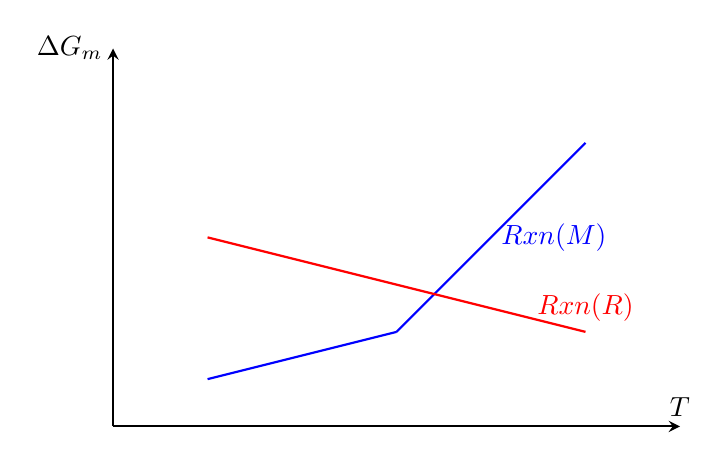
\begin{tikzpicture}[scale=1.2,
                    >=stealth,
                    axis/.style={thick,black}]

\draw[axis,->] (0,0) -- (6,0) node[above] {$T$}; 
\draw[axis,->] (0,0) -- (0,4) node[left] {$\Delta G_m$}; 

\draw[thick,blue] (1,0.5) -- (3,1) node[midway,above right]{};
\draw[thick,blue] (3,1) -- (5,3) node[midway,right] {$Rxn(\text{M})$};
\draw[thick,red] (1,2) -- (5,1) node[right,above] {$Rxn(\text{R})$};

\end{tikzpicture} 
\end{center}

其中斜率为$-\Delta_r S_m$，偏摩尔Gibbs自由能的零点为$T_0 = {\Delta_r H_m}/{\Delta_r S_m}$，其自发的转变温度，即偏摩尔Gibbs自由能小于0以下对应温度是自发的，而对一个耦合的反应，我们还是以金属冶炼为例，还原剂在金属线下是自发。

图中还有一个令人注意的点，即我们的金属线发生了转折，显然这源于熔化，减少了熵变，导致斜率提高。
\end{definition}

\newpage

\section{氧化还原反应与电化学}  
\subsection{氧化还原反应的基本概念}

现在我们进一步推广热力学的部分，即引入非体积功。最简单的是电功，而这样的反应为氧化还原反应。

\begin{definition}[氧化还原反应]
氧化还原反应是涉及电子转移或电子对偏向的化学反应。
\end{definition}

我们这里着重区分氧化数（氧化态）和化合价的概念：
\begin{definition}[氧化数和化合价]
  \begin{enumerate}
    \item 氧化态（$ON$）是指化合物中，假设所有共价键均为离子键（电子归属于电负性更大的原子）时某原子的带电量。
    \item 化合价是指化合物中，某原子成键数量，显然非负。
  \end{enumerate}
\end{definition}

依照这个定义，氧化还原反应可以被定义为氧化态发生变化的反应。

我们往往考察这样的一个反应：$$Red_1 + Ox_2  \to Ox_1 + Red_2$$其中$Ox$和$Red$分别是某物质氧化态和还原态的缩写（我们用角标1，2区分两个物质）。但这相对复杂，我们将其分割：

\begin{definition}[电极半反应]
任何氧化还原反应均可拆分为两个半反应：氧化半反应（失去电子，氧化态升高）和还原半反应（得到电子，氧化态降低）。其一般形式为：
$$Red_1- ze^- \to Ox_1 , \quad Ox_2 + ze^- \to Red_2$$
显然氧化过程失去的电子数等于还原过程得到的电子数（电子守恒）。
\end{definition}

下表给出了相关术语:

\begin{definition}[氧化还原反应相关术语]
\begin{center}
\begin{tabular}{c c c c c}
    \toprule
    反应物氧化数 & 电极半反应 & 反应物 & 行为 & 变化为 \\
    \midrule
    升 & 氧化半反应 & 还原剂 \(Red\) & 被氧化 & 氧化产物 \(OP/Ox'\) \\
    降 & 还原半反应 & 氧化剂 \(Ox\) & 被还原 & 还原产物 \(RP/Red'\) \\
    \bottomrule
\end{tabular}
\end{center}
\end{definition}

\subsection{电极电势}

热力学量是宏观的，而单个化学反应的电子转移是微观的，需要建立联系。

\begin{definition}[Faraday（法拉第）常数]
Faraday常数（$F$）是每摩尔电子所携带的电荷量， $F = N_A e$，其数值约为 $F = 96500\ \mathrm{C\cdot mol^{-1}}$。
\end{definition}

Faraday以实验总结了如下规律，其为电化学的基础：

\begin{proposition}[Faraday电解定律（第一、第二定律）]
\begin{enumerate}
    \item 第一定律：电解过程中，电极上沉积或溶解的物质的量（$n$）与通过电解质溶液的电荷量（$Q$）成正比：$n = {Q}/{zF}$，其中 $z$ 为每个离子转移的电子数。
    \item 第二定律：相同电荷量下，不同物质在电极上沉积的质量与其摩尔质量（$M$）除以转移电子数（$z$）成正比：$\frac{m_1}{m_2} = \frac{M_1/z_1}{M_2/z_2}$。
\end{enumerate}
\end{proposition}

对于电学量的讨论必然涉及电势$\phi $及电势差，我们从一个有趣的事实开始：当金属M制作的电极插入含有金属离子$M^{z+}$的盐溶液中，可能发生金属离子吸附、沉积到电极上，或者电极溶解。在这个过程中，由于电荷的累积，电极与溶液产生了电势差：

\begin{definition}[Trasatti绝对电极电势及其推广]
绝对电极电势是金属电极与盐溶液之间因电极-溶液界面电荷积累产生的电势差。即：
$$\varphi_{abs}(M^{z+}/M)=\phi_M - \phi_{sol}, \quad \varphi_{abs}(Ox/Red) = \phi_{Red} - \phi_{Ox} $$
\end{definition}

然而，这些电势是难测的（注意不是不可测），所以我们定义一个基准：

\begin{definition}[标准氢电极与相对电极电势]
标准氢电极（$SHE$）作为参比电极，其标准电极电势在298.15 K下定义为 $\varphi^\circ(H^+/H_2) = 0\ \mathrm{V}$（100 kPa $H_2$，$1\ \mathrm{mol\cdot L^{-1}}\ H^+$）,其绝对量为：

$$\varphi_{abs}(SHE) = (\varDelta_{hyd}G_m^\circ + IE_1^\circ +\frac{1}{2}BDE)/F + \varphi_{correction} = 4.44\text{V}$$

相对电极电势（$\varphi$）是指被测电极与标准氢电极在指定条件下的电势差。标准电极电势（$\varphi^\circ$）是指标准状态下（纯固/液态、$1\ \mathrm{mol\cdot L^{-1}}$ 溶质、100 kPa气体）的电极电势。
\end{definition}

对于一个两电极的电池，其电动势用花体字母$\mathcal{E}$表示：

\begin{proposition}[电动势]
$$\mathcal{E} = \phi_+ -\phi_- =\varphi_{Ox} - \varphi_{Red}  $$
\end{proposition}

我们回忆第一章的热力学条件，当涉及非体积功时，我们给出了热力学的允许条件，结合电功的定义：$$\Delta G < W_f = q U $$假定Gibbs自由能完全做电功：

\begin{proposition}[电极电势与Gibbs自由能的关系]
电极反应的摩尔吉布斯自由能变与电极电势的关系为：
$$\Delta_r G_m = -zF\mathcal{E} =- z F (\varphi_{Ox} - \varphi_{Red})$$

所以其自发要求氧化半反应电极电势大于还原半反应，也就是说：
\begin{enumerate}
  \item 氧化剂电极电势越大，氧化能力越强；
  \item 还原剂电极电势越小，还原能力越强。
\end{enumerate}
\end{proposition}

电极电势往往应用于元素化学，所以我们很自然地考虑某一个元素，有：

\begin{definition}[Latimer（拉蒂默）标准电极电势图]
Latimer图展示了某元素在特定介质（酸性/碱性）中不同氧化态的标准电极电势，按氧化态从高到低（从左到右）排列。每一个箭头上都标注了箭头两端物质之间的电极电势。

结合我们之前的结论，若某物质右侧半反应的电极电势比左侧更正，则该物种容易发生歧化。
\end{definition}
\begin{example}[氮的Latimer标准电极电势图]
  $$
(pH = 0)\quad\text{NO}_3^- \xrightarrow{0.94\ \text{V}} 
\text{HNO}_2 \xrightarrow{1.00\ \text{V}} 
\text{NO} \xrightarrow{1.59\ \text{V}} 
\text{N}_2\text{O} \xrightarrow{1.77\ \text{V}} 
\text{N}_2 \xrightarrow{-0.23\ \text{V}} 
\text{NH}_4^+
$$


$$
(pH =14)\quad\text{NO}_3^- \xrightarrow{0.01\ \text{V}} 
\text{NO}_2^- \xrightarrow{0.46\ \text{V}} 
\text{NO} \xrightarrow{0.76\ \text{V}} 
\text{N}_2\text{O} \xrightarrow{0.94\ \text{V}} 
\text{N}_2 \xrightarrow{-0.73\ \text{V}} 
\text{NH}_3
$$

\end{example}

Latimer标准电极电势图仅仅提供的相邻氧化态物质之间的电极电势。跨越多个氧化态时，需要注意电极电势不是状态函数，以此不具备加和性：

\begin{proposition}[电极电势的计算]
电极电势不能直接相加，但Gibbs自由能变具有加和性。对于一系列氧化态变化：$$\text{OS}_1 \stackrel{z_1, \varphi_1}{\rightarrow} \text{OS}_2 \stackrel{z_2, \varphi_2}{\rightarrow} \text{OS}_3$$则$\text{OS}_3/\text{OS}_1$的电极电势为：
$$\varphi(\text{OS}_3/\text{OS}_1) = \frac{z_1\varphi_1 + z_2\varphi_2}{z_1 + z_2}$$
其中 $z_1$ 和 $z_2$ 为各步转移的电子数，$\varphi_1$、$\varphi_2$ 为对应的电极电势。
\end{proposition}

Frost（弗罗斯特）-Ebsworth（埃布斯沃思）图，即$z\varphi ^\circ-ON$图（与偏摩尔Gibbs自由能-氧化态图等价）更加直观地展示了这个结果（其中$z$指相对于单质转移的电子数）。类似于Jensen（琴生）不等式，我们只需要将需要的三个物质相连，观察形成的折线。如果是上凸的，则意味着中间的物质易发生歧化；如果是下凹的，则意味着两侧的物质易发生归中。

\begin{example}[氮的Frost-Ebsworth图]
  
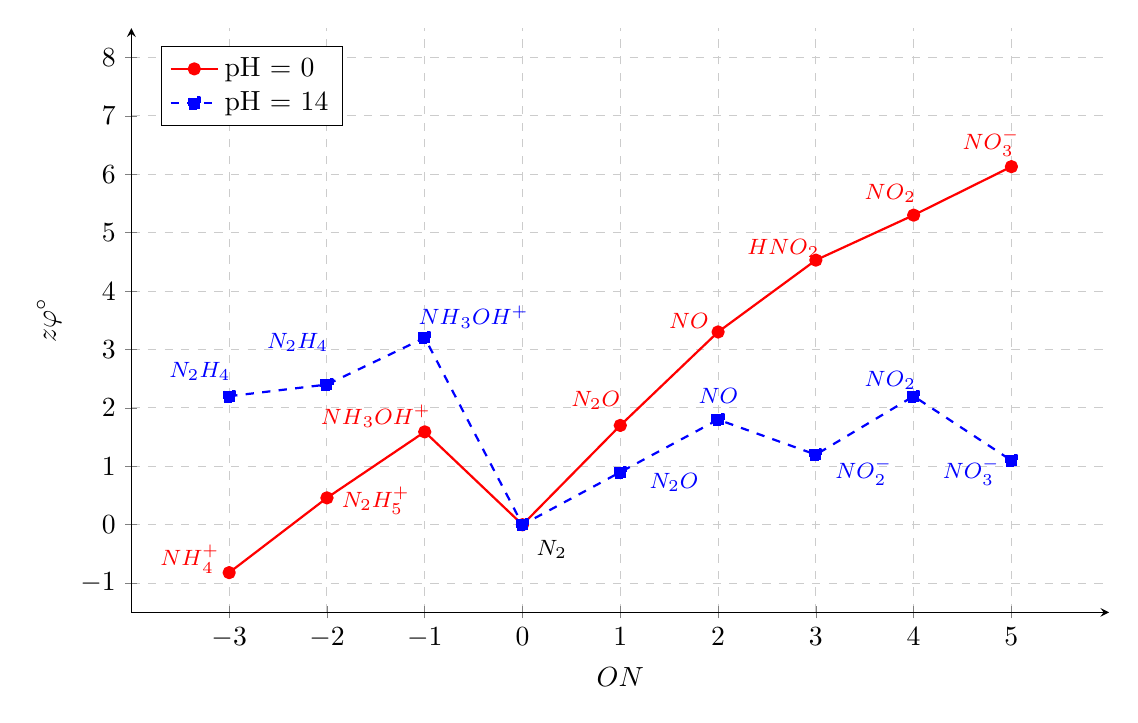
\begin{tikzpicture}
\begin{axis}[
    width=14cm,
    height=9cm,
    xlabel={$ON$},
    ylabel={$z\varphi ^\circ$},
    xmin=-4, xmax=6,
    ymin=-1.5, ymax=8.5,
    xtick={-3,-2,-1,0,1,2,3,4,5},
    ytick={-1,0,1,2,3,4,5,6,7,8},
    grid=major,
    grid style={dashed, gray!40},
    legend pos=north west,
    legend cell align={left},
    axis lines=left,
    enlargelimits=false,
    clip=false,
    every node near coord/.append style={font=\small, anchor=south west},
]



\addplot[
    color=red,
    mark=*,
    thick,
    sharp plot, 
    line join=round
] coordinates {
    (-3, -0.82)  
    (-2, 0.46)  
    (-1, 1.59) 
    (0, 0.00)  
    (1, 1.70) 
    (2, 3.3)
    (3, 4.53)
    (4, 5.3)
    (5, 6.13) 
};
\addlegendentry{pH = 0}

\node[anchor=south east, red, font=\footnotesize] at (axis cs:-3,-1) {$\text{NH}_4^+$};
\node[anchor=south, red, font=\footnotesize] at (axis cs:-1.5,0) {$\text{N}_2\text{H}_5^+$};
\node[anchor=south, red, font=\footnotesize] at (axis cs:-1.5,1.5) {$\text{NH}_3\text{OH}^+$};
\node[anchor=north, black, font=\footnotesize] at (axis cs:0.3,-0.1) {$\text{N}_2$};
\node[anchor=south west, red, font=\footnotesize] at (axis cs:0.4,1.8) {$\text{N}_2\text{O}$};
\node[anchor=south west, red, font=\footnotesize] at (axis cs:1.4,3.2) {$\text{NO}$};
\node[anchor=south west, red, font=\footnotesize] at (axis cs:2.2,4.4) {$\text{HNO}_2$};
\node[anchor=north west, red, font=\footnotesize] at (axis cs:3.4,6) {$\text{NO}_2$};
\node[anchor=south west, red, font=\footnotesize] at (axis cs:4.4,6.13) {$\text{NO}_3^-$};

\addplot[
    color=blue,
    mark=square*,
    thick,
    sharp plot, 
    dashed,
    line join=round
] coordinates {
    (-3, 2.2) 
    (-2, 2.4)  
    (-1, 3.2)  
    (0, 0.00)  
    (1, 0.9)   
    (2, 1.8)  
    (3, 1.2)  
    (4, 2.2) 
    (5, 1.1)    
};
\addlegendentry{pH = 14}
\node[anchor=south, blue, font=\footnotesize] at (axis cs:-3.3,2.3) {$\text{N}_2\text{H}_4$};
\node[anchor=south, blue, font=\footnotesize] at (axis cs:-2.3,2.8) {$\text{N}_2\text{H}_4$};
\node[anchor=south, blue, font=\footnotesize] at (axis cs:-0.5,3.2) {$\text{NH}_3\text{OH}^+$};
\node[anchor=south west, blue, font=\footnotesize] at (axis cs:1.2,0.4) {$\text{N}_2\text{O}$};
\node[anchor=south west, blue, font=\footnotesize] at (axis cs:1.7,1.9) {$\text{NO}$};
\node[anchor=south west, blue, font=\footnotesize] at (axis cs:3.1,0.5) {$\text{NO}_2^-$};
\node[anchor=north west, blue, font=\footnotesize] at (axis cs:3.4,2.8) {$\text{NO}_2$};
\node[anchor=south west, blue, font=\footnotesize] at (axis cs:4.2,0.5) {$\text{NO}_3^-$};

\end{axis}
\end{tikzpicture}

例如，通过连线可以发现：
\begin{enumerate}
  \item 碱性条件下一氧化氮与二氧化氮容易归中，而酸性条件下亚硝酸容易歧化。
  \item 无论是酸性还是碱性，羟胺都容易与亚硝酸（根）归中为氮。
\end{enumerate}

但是如同我们在第一章强调的那样，这是热力学上的允许，而不一定真的发生。

\end{example}

\subsection{条件对电极电势的影响}

我们已经给出了电极电势和Gibbs自由能的关系，结合van't Hoff等温等压方程，给出：

\begin{proposition}[Nernst（能斯特）方程]
$$\varphi = \varphi^\circ - \frac{RT}{zF}\ln\frac{[\text{Red}]}{[\text{Ox}]}$$
298.15 K时，方程简化为：
$$\varphi = \varphi^\circ - \frac{0.0592}{z}\lg\frac{[\text{Red}]}{[\text{Ox}]}$$

所以，最直观地，浓度影响着电极电势：
\begin{enumerate}
    \item 增大 $[\text{Ox}]$、减少$[\text{Red}]$  使 $\varphi$ 升高（氧化性增强）；
    \item 增大 $[\text{Red}]$、减少$[\text{Ox}]$  使 $\varphi$ 降低（还原性增强）。
\end{enumerate}
而且，这种影响对转移电子数更少的反应、在更高的温度更加显著。
\end{proposition}

同样的，沉淀与络合间接地影响着浓度：

\begin{proposition}[沉淀和络合的影响]
\begin{enumerate}
    \item 沉淀：氧化态/还原态形成沉淀会降低其有效浓度，导致氧化态的 $\varphi$ 降低（或还原态的 $\varphi$ 升高）。
    \item 络合：氧化态/还原态形成稳定络合物会降低其有效浓度，效果与沉淀相同。
\end{enumerate}
\end{proposition}

\begin{example}
  \begin{enumerate}
    \item 随着卤族元素（除去可溶的氟化银）半径的增加，卤化银的溶度积逐渐减小，标准状况下（卤离子浓度为标准浓度）银离子电极电势减小，氧化性降低。
    \item 王水溶金的原理：由于 Au$^{3+}$ 与 Cl$^-$ 络合，$\varphi^\circ(\text{Au}^{3+}/\text{Au}) $减小为$ \varphi^\circ(\text{AuCl}_4^-/\text{Au})$，使得硝酸的电极电势大于金的氧化电位，反应可以发生。
  \end{enumerate}
\end{example}

Nernst方程没有直接的酸度项，但是对于某些含H或O和化合物（如含氧酸），其电极反应涉及 H$^+$ 或 OH$^-$ （如 O$_2 + 4\text{H}^+ + 4e^- \to 2\text{H}_2\text{O}$），溶液的pH对电极电势有显著影响。此类反应的能斯特方程包含 $[\text{H}^+]$/$[\text{OH}^-]$ ，对于酸性还原反应，电极电势随pH升高而降低。


\begin{definition}[Pourbaix（普尔贝）图（pH-$\varphi $图）]
Pourbaix图是将氧化还原系统的电极电势（$\varphi$）对溶液pH作图。图中划分了不同物种的稳定区域，并显示了水的氧化（生成 O$_2$）和还原（生成 H$_2$）的条件。在两条水线之间稳定的物种与水相容。然而，由于溶液中电子转移的迟缓效应，我们常常将氢线与氧线向外平移0.5V为稳定线，认为稳定线之间的物质是可以与水共存。
\end{definition}

\begin{example}[Pourbaix图举例]
  \begin{tikzpicture}
\begin{axis}[
    width=14cm,
    height=9cm,
    xlabel={pH},
    ylabel={Eh ($\varphi $ vs. SHE)},
    xmin=0, xmax=14,
    ymin=-1.2, ymax=2.2,
    grid=both,
    minor tick num=1,
    legend pos=north east, 
    legend style={font=\small, cells={anchor=west}},
    every axis plot/.append style={thick},
    tick label style={font=\small},
    label style={font=\small}
]

\addplot[blue, dashed, domain=0:14, samples=100] {0 - 0.0592*x};
\addplot[red, dashed, domain=0:14, samples=100] {1.229 - 0.0592*x};
\addplot[blue, dotted, domain=0:14, samples=100] {0 - 0.0592*x - 0.5};
\addplot[red, dotted, domain=0:14, samples=100] {1.229 - 0.0592*x + 0.5};

\addplot[green!70!black, domain=0:14, samples=100] {1.358};
\addplot[cyan!70!blue, domain=0:14, samples=100] {1.482 - 0.0296*x};
\addplot[magenta!70!red, domain=0:14, samples=100] {1.451 - 0.0592*x};
\addplot[orange!80!red, domain=0:14, samples=100] {0.957 - 0.0789*x};
\addplot[purple!70!blue, domain=0:14, samples=100] {0.803 - 0.1184*x};
\addplot[brown!80!black, domain=0:14, samples=100] {1.507 - 0.0947*x};
\addplot[teal!70!green, domain=0:14, samples=100] {1.679 - 0.0789*x};
\legend{
    氢线 (H$^+$/H$_2$),
    氧线 (O$_2$/H$_2$O),
    氢稳定线,
    氧稳定线,
    Cl$_2$/Cl$^-$,
    HClO/Cl$^-$,
    ClO$_3^-$/Cl$^-$,
    NO$_3^-$/NO,
    NO$_3^-$/NO$_2$,
    MnO$_4^-$/Mn$^{2+}$,
    MnO$_4^-$/MnO$_2$
}
\end{axis}
\end{tikzpicture}

总体而言，电极电势随pH线性降低，但对于不涉及$\text{H}^+$/$\text{OH}^-$ 的反应，其图像为水平直线。
\end{example}

\newpage

\section{化学动力学}
\subsection{反应速率与速率方程}
从动力学开始，我们开始讨论反应的快慢，类比力学，我们将一般反应 $aA + bB \rightarrow cC + dD$的平均反应速率$\langle rate \rangle$定义为某一反应物或产物的浓度在单位时间间的变化，瞬时速率为其极限：
\begin{definition}[反应速率]
$$\langle rate \rangle = \frac{\Delta c}{\Delta t}$$
$$rate = \lim_{\Delta t \to 0} \frac{\Delta c}{\Delta t} = \frac{dc}{dt}$$
归一化后，统一反应速率为：
$$rate = -\frac{1}{a}\frac{d[\text{A}]}{dt} = -\frac{1}{b}\frac{d[\text{B}]}{dt} = \frac{1}{c}\frac{d[\text{C}]}{dt} = \frac{1}{d}\frac{d[\text{D}]}{dt} > 0$$
负号表示反应物浓度随时间降低。
\end{definition}

而对于整体的反应而言，大量实验总结了化学反应速率与反应物浓度关联的方程：

\begin{definition}[动力实验方程]
化学反应开始时的速率与反应物的幂次成正比，：
$$rate = k_{m+n}[\text{A}]^m[\text{B}]^n$$
其中 $k$ 为速率常数，幂次$m$ 和 $n$ 为对反应物A和B的反应级数），总反应级数为 $m + n$。
\end{definition}

结合速率的定义，我们可以建立微分方程（微分速率定律），解得反应物浓度随时间变化的方程（积分速率定律），例如：

对于不可逆一级反应：

$$\text{A} \xrightarrow{k} \text{P}$$反应速率定义为反应物A的消耗速率，微分形式为：
$$-\frac{\text{d}[\text{A}]}{\text{d}t} = k[\text{A}]$$将微分方程分离变量：
$$\frac{\text{d}[\text{A}]}{[\text{A}]} = -k \text{d}t$$对两边积分：
\begin{align*}
\int_{[\text{A}]_0}^{[\text{A}]} \frac{\text{d}[\text{A}]}{[\text{A}]} &= -k \int_{0}^{t} \text{d}t \\
\end{align*}
即可得到积分速率定律：
$$ln[\text{A}] = \ln[\text{A}]_0 - kt$$
令$[\text{A}]=1/2[\text{A}]_0$，可得半衰期\(t_{1/2} = \frac{\ln 2}{k_1}\)。

同理可以计算其他情况，给出下表：

\begin{proposition}[零级、一级和二级反应的动力学特征]
对于单反应物不可逆反应 $\text{A} \rightarrow \text{P}$，往往是零级、一级或二级反应，其重要的相关结果如下（其中 $[A]_0$ 为A的初始浓度）：
   
\begin{center}
\begin{tabular}{c c c c c}
    \toprule
    反应级数 & 微分速率定律 & 积分速率定律 & 半衰期 \(t_{1/2}\) & 情况 \\
    \midrule
    零级反应 & \(v = k_0\) & \([\text{A}] = [\text{A}]_0 - k_0 t\) & \(t_{1/2} = \frac{[\text{A}]_0}{2k_0}\) & 大多数气-固表面过程 \\
    一级反应 & \(v = k_1 [\text{A}]\) & \(\ln[\text{A}] = \ln[\text{A}]_0 - k_1 t\) & \(t_{1/2} = \frac{\ln 2}{k_1}\) & 重排、衰变、热分解 \\
    二级反应 & \(v = k_2 [\text{A}]^2\) & \(\frac{1}{[\text{A}]} = \frac{1}{[\text{A}]_0} + k_2 t\) & \(t_{1/2} = \frac{1}{k_2 [\text{A}]_0}\) & / \\
    \bottomrule
\end{tabular}
\end{center}
值得注意的是，零级反应的速率以及一级反应的半衰期是定值。

\end{proposition}

\subsection{碰撞理论与反应机理}

现在，我们从经验科学转至理论科学，以一种偏公理化的风格介绍碰撞理论：

\begin{definition}[碰撞理论]
\begin{enumerate}
  \item 化学反应的实质是分子之间的碰撞；
  \item 碰撞不一定是有效的，除非是特定能量区间的分子在合适取向下的碰撞；
\end{enumerate}
\end{definition}

现在，我们逐步剖析上述概念，首先是碰撞频率，由Maxwell分布导出：$$Z_{\text{AB}} = n_{\text{A}} n_{\text{B}} \sigma_{AB}\sqrt{\frac{8 k_B T}{\mu \pi} }$$其中$n$为分子数密度；$\sigma$是有效碰撞面积，$\pi(r_{\text{A}}^2+r_{\text{B}}^2)$；$\mu$为约化质量，$(\frac{1}{m_{\text{A}}}+\frac{1}{m_{\text{B}}})^{-1}$；$k_B$为Boltzmann常量。显然，碰撞频率与密度（浓度）、面积、温度正相关，与 质量负相关。

其次是所谓的能量合适，我们称能量在该区间的分子为活化分子，用双剑标$\ddagger$标注，在这个基础上，我们定义：

\begin{definition}[Tolman活化能]
活化能$E_a$定义为活化分子的平均能量与所有反应物分子的平均摩尔能量之差：$$ E_a = \left(\langle \varepsilon ^\ddagger \rangle - \langle \varepsilon  \rangle\right)N_A$$
依照这个定义，正逆反应活化能之差为能量变。
\end{definition}

值得注意的是，我们表述的是“特定能量区间”而非“大于某个值”（类比将粘性球投掷在墙上，反而因为速度过大而反弹了）。所以，活化能可能为负，特别是在反应物高度活泼（比如自由基）的情况下。

我们按照最经典的情况，即“能量大于某个值”，Boltzmann分布给出了该区间的分子权重，$$f = \exp (-\frac{E_a}{RT})$$

最后，我们用$P$表示分子碰撞时合适取向的概率，越大的分子，越小的反应位点，其值越小。事实上，$P$也是能量的函数，这里高度简化了。

我们将上述因子相乘：

\begin{proposition}[有效碰撞频率]
有效碰撞频率（$Z_{\text{eff}}$）是指单位体积单位时间内的有效碰撞次数，计算公式为：
$$Z_{\text{eff}} = n_{\text{A}} n_{\text{B}} \sigma_{\text{AB}} P \sqrt{\frac{8 k_B T}{\mu \pi} } \exp (-\frac{E_a}{RT})$$
\end{proposition}

而在此之前，实验给出了如下的经验公式，相比于指数项，根号内的温度对速率影响较小，以至于当时实验几乎无法观测。出于同样的理由，也是一个良好的近似。

\begin{proposition}[Arrhenius经验方程]
$$k = A\exp\left(-\frac{E_a}{RT}\right)$$
其中 $A$ 为指前因子。
\end{proposition}


这样的的一次碰撞产生了一个化学反应，是一个简单的过程：

\begin{definition}[基元反应与反应机理]
基元反应是一步完成的化学反应，在碰撞理论下可以被理解为一次有效碰撞。（参与分子数往往小于等于二，除非某些分子数密度极大，比如溶剂）

反应机理是即一系列基元反应的按序罗列。
\end{definition}

化学反应的实质是电子云的流动。一般地，我们可以用弯曲箭头代表一对电子的流动（单箭头表示一个电子），用以表示机理。

显然，电子倾向于从高能状态向低能状态演化（以下参见第四章）：

\begin{definition}[亲核试剂与亲电试剂]
  \begin{enumerate}
    \item 亲核试剂$Nu$是电子对的给体，往往具有较高的$HOMO$；
    \item 亲电试剂$E$是电子对的受体，往往具有较高的$LUMO$。
  \end{enumerate}
\end{definition}
于是，箭头从亲核试剂出发打向亲电试剂。

依照之前的讨论，碰撞频率正比于分子数密度，自然也正比于浓度，所以我们可以强化其动力实验方程：

\begin{proposition}[质量作用定律]
对于基元反应 $a\text{A} + b\text{B} +c\text{C}\rightarrow \text{产物}$，动力实验方程可直接根据反应物的计量系数写出：
$$rate = k[\text{A}]^a[\text{B}]^b[\text{C}]^c$$
\end{proposition}

\subsection{过渡态理论与决速步}

一个基元反应在反应进程-势能图上往往是一个先升后降的曲线，我们给曲线的各个部分命名如下：

\begin{definition}[活化络合物]
\begin{enumerate}
  \item 始态（$S.M.$）：势能图的起点;
  \item 终态（$pdts.$）：势能图的终点；
  \item 过渡态（$T.S.$）：势能图的最高点，又称活化络合物。
\end{enumerate}
\end{definition}
例如，对于基元反应 $\text{A}-\text{B} + \text{C} \rightarrow [\text{A}\cdots \text{B}\cdots \text{C}]^\ddagger \rightarrow \text{A} + \text{B}-\text{C}$，$[\text{A}\cdots \text{B}\cdots \text{C}]^\ddagger$ 为活化络合物。

过渡态与反应物之间的（摩尔）能量差为能垒（$E_0$），依照定义，这是一个非负的数值。我们往往认为其与活化能近似相等。下文混用活化能与能垒。

对于多步反应，中间体（$ints$）是两个过渡态之间势能最低点的称谓。一个复杂反应可以表示为：$$S.M.\longrightarrow T.S_1 \longrightarrow ints_1\longrightarrow T.S_2\longrightarrow ...\longrightarrow T.S_n \longrightarrow pdts.$$其中的每一步都可以写出质量作用定律。然而各个步骤的贡献并不相同，正如木桶效应表示的那样，慢步骤决定了整体的速率。

例如：一氧化氮的氧化反应，其机理为：$$2\text{NO} + \text{O}_2 \longrightarrow [\text{NO} \cdots \text{NO}]^ \ddagger + \text{O}_2 \longrightarrow \text{N}_2\text{O}_2 + \text{O}_2 \longrightarrow  [\text{N}_2\text{O}_2 \cdots \text{O}_2]^\ddagger \longrightarrow 2\text{NO}_2 $$

\begin{definition}[决速步]
决速步（RDS）是多步反应机理中速率最小的基元反应，这往往意味着活化能最大。总反应的速率由决速步的速率决定，因为它是机理中最慢的步骤。
\end{definition}

在复杂反应的速率方程确定过程中，往往采取近似的方法，即平衡态近似与稳态近似：

\begin{proposition}[平衡态近似]
对于快速可逆步骤后接慢速速控步的反应机理，假设快速步骤处于快速预平衡（正、逆反应速率相等）。根据平衡常数计算快速步骤生成的中间物种浓度，再代入慢速步骤的速率方程，推导总速率定律（经验速率方程）。
\end{proposition}

\begin{example}[一氧化氮氧化过程的速率方程计算（平衡态近似）]
一氧化氮氧化过程分为两步：

1. 快：$2\text{NO} \rightleftharpoons  \text{N}_2\text{O}_2$：$k_{1}$，$k_{-1}$

2. 慢：$\text{N}_2\text{O}_2 + \text{O}_2 \longrightarrow 2\text{NO}_2$：$k_2$

快反应正逆反应平衡，此时：

$$k_1[\text{NO}]^2 = k_{-1}[\text{N}_2\text{O}_2] \quad K = \frac{k_1}{k_{-1}} = \frac{[\text{N}_2\text{O}_2]}{[\text{NO}]^2}$$
总反应速率由慢步骤决定：

$$rate = k_2 [\text{N}_2\text{O}_2][\text{O}_2]$$
将 $[\text{N}_2\text{O}_2]$ 代入速率方程：

$$rate = k_2 \cdot \frac{k_1}{k_{-1}} [\text{NO}]^2 [\text{O}_2]$$
令表观速率常数 $k^{obs} = k_1 k_2/k_{-1}$，简化得：

$$rate = k^{obs} [\text{NO}]^2 [\text{O}_2]$$
\end{example}

除此之外，有一些反应无法假设平衡，此时可以使用：

\begin{proposition}[稳态近似]
某些反应过程中，假设中间产物的生成速率等于消耗速率，即中间产物的浓度随时间保持恒定。尤其适用于中间物浓度极低且变化极慢的反应。
\end{proposition}

\begin{example}[一氧化氮氧化过程的速率方程计算（稳态近似）]
反应中，$\text{N}_2\text{O}_2$是中间体，其浓度近似不变，即：
$$\frac{d[\text{N}_2\text{O}_2]}{dt} = k_1[\text{NO}]^2 - k_{-1}[\text{N}_2\text{O}_2] - k_2[\text{N}_2\text{O}_2][\text{O}_2] = 0$$
解得：

$$[\text{N}_2\text{O}_2] = \frac{k_1[\text{NO}]^2}{k_{-1} + k_2[\text{O}_2]}$$
带入得:

$$rate = k_2[\text{N}_2\text{O}_2][\text{O}_2] = \frac{k_1k_2[\text{NO}]^2[\text{O}_2]}{k_{-1} + k_2[\text{O}_2]}$$

\end{example}

相比于平衡态近似，稳态近似要求较少，适用范围更广，但是计算相应较为繁琐。
\subsection{条件对化学反应速率的影响}

从Arrhenius方程可以看出，$A$、$E_a$、$T$是影响化学反应速率常数的典型物理量，我们将分别讨论。

首先是指前因子，其与碰撞相关，这里只罗列两种：

\begin{proposition}[改变指前因子]
  \begin{enumerate}
    \item 接触面积：对于非均相反应，接触面积大（碾碎、超声）会显著提高反应速率；
    \item 同位素效应：质量大的同位素有更大的约化质量，导致碰撞频率降低，体现为不活泼。
  \end{enumerate}
\end{proposition}

其次是活化能，分为改变反应路径和改变分子势能两种：

\begin{proposition}[改变活化能]
  \begin{enumerate}
    \item 催化剂：改变反应路径以改变活化能，典型的比如酶促反应；
    \item 极性：化学反应中间体往往是离子，其在大极性溶剂更加稳定。
  \end{enumerate}
\end{proposition}

\begin{example}[指前因子和活化能]
  \begin{enumerate}
    \item 重排反应中，处于相同化学环境的$\text{H}$总是比$\text{D}$优先发生重排；
    \item 叔丁基溴与氢氧化钠反应，在乙醇中反应速度显著快于丙酮。
  \end{enumerate}
\end{example}

值得注意的是温度。一般而言，温度越高，化学反应速率越快。然而，在一些情况恰恰相反，产生所谓的“负温度效应”。第一种情况是是改变温度后改变了反应路径（最经典的即酶促反应的失活），不再赘述。第二种情况为活化能为负，比如二氧化氮的二聚。但是出于同样的原因，反应速度极快，难以观测。

活化能为基元反应的概念，但对于一个已知速率方程的反应，我们通过拼凑Arrhenius方程的方法计算得到“表观活化能$E_a^{obs}$”：

\begin{example}[一氧化氮氧化（平衡态近似）的表观活化能]
注意到表观反应速率常数的表达式：
$$k^{obs} = \frac{k_1 k_2}{k_{-1}}$$
结合$k_1 = A_1 e^{-E_{a1}/(RT)}, \quad k_{-1} = A_{-1} e^{-E_{a(-1)}/(RT)}, \quad k_2 = A_2 e^{-E_{a2}/(RT)} $
整理得：
$$k^{obs} = \frac{A_1 A_2}{A_{-1}} e^{-(E_{a1} + E_{a2} - E_{a(-1)})/(RT)}$$
我们只关心活化能部分：
$$E_a^{obs} = E_{a1} + E_{a2} - E_{a(-1)}$$
\end{example}

不难发现，如果$E_{a(-1)}$较大，反应的表观活化能为负。这也比较好理解，若表观活化能为负（默认各个反应活化能为正），则$E_{a(-1)}$必定大于$E_{a(1)}$，快反应焓变为负，在升温时平衡逆向移动。

\newpage

\section{原子结构与化学键}
\subsection{Bohr原子模型}
\subsection{元素周期律}
\subsection{价键理论}
\subsection{分子轨道理论}
\subsection{离域键}
\subsection{稳定性判据}

\newpage

\section{晶体结构}
\subsection{晶格与晶胞}
\subsection{金属晶体与密堆积}
\subsection{离子晶体与半径比规则}
\subsection{分子晶体与分子间作用力}
\subsection{晶体的性质}

\newpage

\section{配位化合物}
\subsection{配位化合物的基本概念}
\subsection{价键法}
\subsection{晶体场理论}
\subsection{效应与应用}

\newpage

\section{进阶专题}
\subsection{化学热力学进阶专题}
\subsubsection{液体与溶液的性质}
\subsubsection{卡诺循环}
\subsubsection{酸碱与离子平衡}
\subsubsection{化学势}

\newpage
\subsection{氧化还原反应与电化学进阶专题}
\subsubsection{电化学势}
\subsubsection{过电势}

\newpage
\subsection{化学动力学进阶专题}
\subsubsection{态-态反应能量变化}
\subsubsection{过渡态理论速率方程}
\subsubsection{竞争反应}
\subsubsection{复杂反应}

\newpage
\subsection{原子结构与化学键进阶专题}
\subsubsection{箱中粒子模型}
\subsubsection{两种方法（VB与MO）的修正}
\subsubsection{分子对称性}

\newpage
\subsection{晶体结构进阶专题}
\subsubsection{准晶}

\newpage
\subsection{配位化合物进阶专题}
\subsubsection{配体场理论}
\subsubsection{超分子化学}

\end{document}